\documentclass[twoside]{book}

% Packages required by doxygen
\usepackage{calc}
\usepackage{doxygen}
\usepackage{graphicx}
\usepackage[utf8]{inputenc}
\usepackage{makeidx}
\usepackage{multicol}
\usepackage{multirow}
\usepackage{textcomp}
\usepackage[table]{xcolor}

% Font selection
\usepackage[T1]{fontenc}
\usepackage{mathptmx}
\usepackage[scaled=.90]{helvet}
\usepackage{courier}
\usepackage{amssymb}
\usepackage{sectsty}
\renewcommand{\familydefault}{\sfdefault}
\allsectionsfont{%
  \fontseries{bc}\selectfont%
  \color{darkgray}%
}
\renewcommand{\DoxyLabelFont}{%
  \fontseries{bc}\selectfont%
  \color{darkgray}%
}

% Page & text layout
\usepackage{geometry}
\geometry{%
  a4paper,%
  top=2.5cm,%
  bottom=2.5cm,%
  left=2.5cm,%
  right=2.5cm%
}
\tolerance=750
\hfuzz=15pt
\hbadness=750
\setlength{\emergencystretch}{15pt}
\setlength{\parindent}{0cm}
\setlength{\parskip}{0.2cm}
\makeatletter
\renewcommand{\paragraph}{%
  \@startsection{paragraph}{4}{0ex}{-1.0ex}{1.0ex}{%
    \normalfont\normalsize\bfseries\SS@parafont%
  }%
}
\renewcommand{\subparagraph}{%
  \@startsection{subparagraph}{5}{0ex}{-1.0ex}{1.0ex}{%
    \normalfont\normalsize\bfseries\SS@subparafont%
  }%
}
\makeatother

% Headers & footers
\usepackage{fancyhdr}
\pagestyle{fancyplain}
\fancyhead[LE]{\fancyplain{}{\bfseries\thepage}}
\fancyhead[CE]{\fancyplain{}{}}
\fancyhead[RE]{\fancyplain{}{\bfseries\leftmark}}
\fancyhead[LO]{\fancyplain{}{\bfseries\rightmark}}
\fancyhead[CO]{\fancyplain{}{}}
\fancyhead[RO]{\fancyplain{}{\bfseries\thepage}}
\fancyfoot[LE]{\fancyplain{}{}}
\fancyfoot[CE]{\fancyplain{}{}}
\fancyfoot[RE]{\fancyplain{}{\bfseries\scriptsize Generated on Mon Jan 13 2014 15\-:51\-:59 for Ontology\-Wrapper by Doxygen }}
\fancyfoot[LO]{\fancyplain{}{\bfseries\scriptsize Generated on Mon Jan 13 2014 15\-:51\-:59 for Ontology\-Wrapper by Doxygen }}
\fancyfoot[CO]{\fancyplain{}{}}
\fancyfoot[RO]{\fancyplain{}{}}
\renewcommand{\footrulewidth}{0.4pt}
\renewcommand{\chaptermark}[1]{%
  \markboth{#1}{}%
}
\renewcommand{\sectionmark}[1]{%
  \markright{\thesection\ #1}%
}

% Indices & bibliography
\usepackage{natbib}
\usepackage[titles]{tocloft}
\setcounter{tocdepth}{3}
\setcounter{secnumdepth}{5}
\makeindex

% Hyperlinks (required, but should be loaded last)
\usepackage{ifpdf}
\ifpdf
  \usepackage[pdftex,pagebackref=true]{hyperref}
\else
  \usepackage[ps2pdf,pagebackref=true]{hyperref}
\fi
\hypersetup{%
  colorlinks=true,%
  linkcolor=blue,%
  citecolor=blue,%
  unicode%
}

% Custom commands
\newcommand{\clearemptydoublepage}{%
  \newpage{\pagestyle{empty}\cleardoublepage}%
}


%===== C O N T E N T S =====

\begin{document}

% Titlepage & ToC
\hypersetup{pageanchor=false}
\pagenumbering{roman}
\begin{titlepage}
\vspace*{7cm}
\begin{center}%
{\Large Ontology\-Wrapper \\[1ex]\large 1.\-0 }\\
\vspace*{1cm}
{\large Generated by Doxygen 1.8.6}\\
\vspace*{0.5cm}
{\small Mon Jan 13 2014 15:51:59}\\
\end{center}
\end{titlepage}
\clearemptydoublepage
\tableofcontents
\clearemptydoublepage
\pagenumbering{arabic}
\hypersetup{pageanchor=true}

%--- Begin generated contents ---
\chapter{Hierarchical Index}
\section{Class Hierarchy}
This inheritance list is sorted roughly, but not completely, alphabetically\-:\begin{DoxyCompactList}
\item Array\-Object\begin{DoxyCompactList}
\item \contentsline{section}{Ontology\-Wrapper\textbackslash{}Container\-Object}{\pageref{class_ontology_wrapper_1_1_container_object}}{}
\begin{DoxyCompactList}
\item \contentsline{section}{Ontology\-Wrapper\textbackslash{}Dictionary\-Object}{\pageref{class_ontology_wrapper_1_1_dictionary_object}}{}
\begin{DoxyCompactList}
\item \contentsline{section}{Ontology\-Wrapper\textbackslash{}Dictionary}{\pageref{class_ontology_wrapper_1_1_dictionary}}{}
\begin{DoxyCompactList}
\item \contentsline{section}{Ontology\-Wrapper\textbackslash{}Wrapper}{\pageref{class_ontology_wrapper_1_1_wrapper}}{}
\end{DoxyCompactList}
\end{DoxyCompactList}
\item \contentsline{section}{Ontology\-Wrapper\textbackslash{}Ontology\-Object}{\pageref{class_ontology_wrapper_1_1_ontology_object}}{}
\begin{DoxyCompactList}
\item \contentsline{section}{Ontology\-Wrapper\textbackslash{}Connection\-Object}{\pageref{class_ontology_wrapper_1_1_connection_object}}{}
\begin{DoxyCompactList}
\item \contentsline{section}{Ontology\-Wrapper\textbackslash{}Collection\-Object}{\pageref{class_ontology_wrapper_1_1_collection_object}}{}
\begin{DoxyCompactList}
\item \contentsline{section}{Ontology\-Wrapper\textbackslash{}Mongo\-Collection}{\pageref{class_ontology_wrapper_1_1_mongo_collection}}{}
\end{DoxyCompactList}
\item \contentsline{section}{Ontology\-Wrapper\textbackslash{}Database\-Object}{\pageref{class_ontology_wrapper_1_1_database_object}}{}
\begin{DoxyCompactList}
\item \contentsline{section}{Ontology\-Wrapper\textbackslash{}Mongo\-Database}{\pageref{class_ontology_wrapper_1_1_mongo_database}}{}
\end{DoxyCompactList}
\item \contentsline{section}{Ontology\-Wrapper\textbackslash{}Server\-Object}{\pageref{class_ontology_wrapper_1_1_server_object}}{}
\begin{DoxyCompactList}
\item \contentsline{section}{Ontology\-Wrapper\textbackslash{}Mongo\-Server}{\pageref{class_ontology_wrapper_1_1_mongo_server}}{}
\end{DoxyCompactList}
\end{DoxyCompactList}
\item \contentsline{section}{Ontology\-Wrapper\textbackslash{}Persistent\-Object}{\pageref{class_ontology_wrapper_1_1_persistent_object}}{}
\begin{DoxyCompactList}
\item \contentsline{section}{Ontology\-Wrapper\textbackslash{}Edge}{\pageref{class_ontology_wrapper_1_1_edge}}{}
\item \contentsline{section}{Ontology\-Wrapper\textbackslash{}Node}{\pageref{class_ontology_wrapper_1_1_node}}{}
\item \contentsline{section}{Ontology\-Wrapper\textbackslash{}Tag}{\pageref{class_ontology_wrapper_1_1_tag}}{}
\item \contentsline{section}{Ontology\-Wrapper\textbackslash{}Term}{\pageref{class_ontology_wrapper_1_1_term}}{}
\end{DoxyCompactList}
\end{DoxyCompactList}
\end{DoxyCompactList}
\end{DoxyCompactList}
\end{DoxyCompactList}

\chapter{Class Index}
\section{Class List}
Here are the classes, structs, unions and interfaces with brief descriptions\-:\begin{DoxyCompactList}
\item\contentsline{section}{\hyperlink{class_ontology_wrapper_1_1_collection_object}{Ontology\-Wrapper\textbackslash{}\-Collection\-Object} }{\pageref{class_ontology_wrapper_1_1_collection_object}}{}
\item\contentsline{section}{\hyperlink{class_ontology_wrapper_1_1_connection_object}{Ontology\-Wrapper\textbackslash{}\-Connection\-Object} }{\pageref{class_ontology_wrapper_1_1_connection_object}}{}
\item\contentsline{section}{\hyperlink{class_ontology_wrapper_1_1_container_object}{Ontology\-Wrapper\textbackslash{}\-Container\-Object} }{\pageref{class_ontology_wrapper_1_1_container_object}}{}
\item\contentsline{section}{\hyperlink{class_ontology_wrapper_1_1_database_object}{Ontology\-Wrapper\textbackslash{}\-Database\-Object} }{\pageref{class_ontology_wrapper_1_1_database_object}}{}
\item\contentsline{section}{\hyperlink{class_ontology_wrapper_1_1_edge}{Ontology\-Wrapper\textbackslash{}\-Edge} }{\pageref{class_ontology_wrapper_1_1_edge}}{}
\item\contentsline{section}{\hyperlink{class_ontology_wrapper_1_1_edge_object}{Ontology\-Wrapper\textbackslash{}\-Edge\-Object} }{\pageref{class_ontology_wrapper_1_1_edge_object}}{}
\item\contentsline{section}{\hyperlink{class_ontology_wrapper_1_1_mongo_collection}{Ontology\-Wrapper\textbackslash{}\-Mongo\-Collection} }{\pageref{class_ontology_wrapper_1_1_mongo_collection}}{}
\item\contentsline{section}{\hyperlink{class_ontology_wrapper_1_1_mongo_database}{Ontology\-Wrapper\textbackslash{}\-Mongo\-Database} }{\pageref{class_ontology_wrapper_1_1_mongo_database}}{}
\item\contentsline{section}{\hyperlink{class_ontology_wrapper_1_1_mongo_server}{Ontology\-Wrapper\textbackslash{}\-Mongo\-Server} }{\pageref{class_ontology_wrapper_1_1_mongo_server}}{}
\item\contentsline{section}{\hyperlink{class_ontology_wrapper_1_1_node}{Ontology\-Wrapper\textbackslash{}\-Node} }{\pageref{class_ontology_wrapper_1_1_node}}{}
\item\contentsline{section}{\hyperlink{class_ontology_wrapper_1_1_node_object}{Ontology\-Wrapper\textbackslash{}\-Node\-Object} }{\pageref{class_ontology_wrapper_1_1_node_object}}{}
\item\contentsline{section}{\hyperlink{class_ontology_wrapper_1_1_ontology_object}{Ontology\-Wrapper\textbackslash{}\-Ontology\-Object} }{\pageref{class_ontology_wrapper_1_1_ontology_object}}{}
\item\contentsline{section}{\hyperlink{class_ontology_wrapper_1_1_server_object}{Ontology\-Wrapper\textbackslash{}\-Server\-Object} }{\pageref{class_ontology_wrapper_1_1_server_object}}{}
\item\contentsline{section}{\hyperlink{class_ontology_wrapper_1_1_tag}{Ontology\-Wrapper\textbackslash{}\-Tag} }{\pageref{class_ontology_wrapper_1_1_tag}}{}
\item\contentsline{section}{\hyperlink{class_ontology_wrapper_1_1_tag_cache}{Ontology\-Wrapper\textbackslash{}\-Tag\-Cache} }{\pageref{class_ontology_wrapper_1_1_tag_cache}}{}
\item\contentsline{section}{\hyperlink{class_ontology_wrapper_1_1_tag_cache_object}{Ontology\-Wrapper\textbackslash{}\-Tag\-Cache\-Object} }{\pageref{class_ontology_wrapper_1_1_tag_cache_object}}{}
\item\contentsline{section}{\hyperlink{class_ontology_wrapper_1_1_tag_object}{Ontology\-Wrapper\textbackslash{}\-Tag\-Object} }{\pageref{class_ontology_wrapper_1_1_tag_object}}{}
\item\contentsline{section}{\hyperlink{class_ontology_wrapper_1_1_term}{Ontology\-Wrapper\textbackslash{}\-Term} }{\pageref{class_ontology_wrapper_1_1_term}}{}
\item\contentsline{section}{\hyperlink{class_ontology_wrapper_1_1_term_object}{Ontology\-Wrapper\textbackslash{}\-Term\-Object} }{\pageref{class_ontology_wrapper_1_1_term_object}}{}
\item\contentsline{section}{\hyperlink{class_ontology_wrapper_1_1_wrapper}{Ontology\-Wrapper\textbackslash{}\-Wrapper} }{\pageref{class_ontology_wrapper_1_1_wrapper}}{}
\end{DoxyCompactList}

\chapter{Class Documentation}
\hypertarget{class_ontology_wrapper_1_1_document_object}{\section{Ontology\-Wrapper\textbackslash{}Document\-Object Class Reference}
\label{class_ontology_wrapper_1_1_document_object}\index{Ontology\-Wrapper\textbackslash{}\-Document\-Object@{Ontology\-Wrapper\textbackslash{}\-Document\-Object}}
}


Inheritance diagram for Ontology\-Wrapper\textbackslash{}Document\-Object\-:
\nopagebreak
\begin{figure}[H]
\begin{center}
\leavevmode
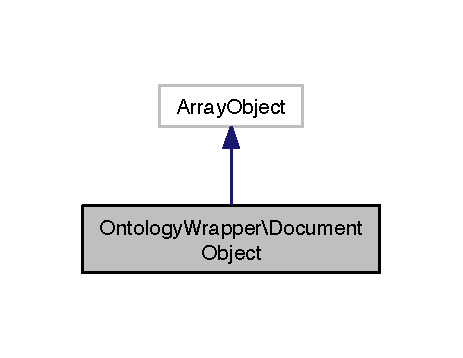
\includegraphics[width=222pt]{class_ontology_wrapper_1_1_document_object__inherit__graph}
\end{center}
\end{figure}


Collaboration diagram for Ontology\-Wrapper\textbackslash{}Document\-Object\-:
\nopagebreak
\begin{figure}[H]
\begin{center}
\leavevmode
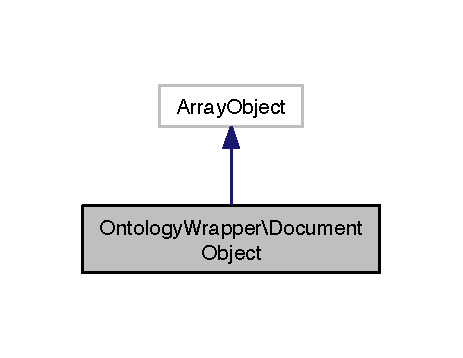
\includegraphics[width=222pt]{class_ontology_wrapper_1_1_document_object__coll__graph}
\end{center}
\end{figure}
\subsection*{Public Member Functions}
\begin{DoxyCompactItemize}
\item 
\hyperlink{class_ontology_wrapper_1_1_document_object_a6d2076d551d0b7035a279bb89db26bd7}{\-\_\-\-\_\-construct} (\$the\-Input=\mbox{[}$\,$\mbox{]}, \$the\-Flags=0, \$the\-Iterator=\char`\"{}Array\-Iterator\char`\"{})
\item 
\hyperlink{class_ontology_wrapper_1_1_document_object_a034f55170eb880dd210f0c9ab15233bc}{offset\-Get} (\$the\-Offset)
\item 
\hyperlink{class_ontology_wrapper_1_1_document_object_aa2e3a251dd102f8aba0645b405a16053}{offset\-Set} (\$the\-Offset, \$the\-Value)
\item 
\hyperlink{class_ontology_wrapper_1_1_document_object_a834adbf7c1f027c3f817dbcf4f12de2d}{offset\-Unset} (\$the\-Offset)
\item 
\hyperlink{class_ontology_wrapper_1_1_document_object_a1d497371592ce2600533565cfaae91b8}{get\-Array\-Copy} ()
\item 
\hyperlink{class_ontology_wrapper_1_1_document_object_a4a96a40abe667d9c3ac7a5d5675dece5}{array\-Keys} ()
\item 
\hyperlink{class_ontology_wrapper_1_1_document_object_ab8e04acc8c14acbeae6d530a604b676a}{array\-Values} ()
\item 
\hyperlink{class_ontology_wrapper_1_1_document_object_a685ca256ab347244104f444cc38362e5}{\-\_\-resolve\-Offset} (\$the\-Offset)
\end{DoxyCompactItemize}
\subsection*{Public Attributes}
\begin{DoxyCompactItemize}
\item 
\hypertarget{class_ontology_wrapper_1_1_document_object_a7bc4d58386184b8f007ad83c6d86e52b}{const {\bfseries k\-T\-A\-G\-\_\-\-N\-I\-D} = '\-\_\-id'}\label{class_ontology_wrapper_1_1_document_object_a7bc4d58386184b8f007ad83c6d86e52b}

\end{DoxyCompactItemize}
\subsection*{Static Public Attributes}
\begin{DoxyCompactItemize}
\item 
\hypertarget{class_ontology_wrapper_1_1_document_object_afd8a2bd1ce090ac17bfe79fc0e596c96}{static {\bfseries \$s\-Tag\-Cache} = N\-U\-L\-L}\label{class_ontology_wrapper_1_1_document_object_afd8a2bd1ce090ac17bfe79fc0e596c96}

\end{DoxyCompactItemize}


\subsection{Detailed Description}
\subparagraph*{Document object}

This class represents the main building block of this library, it implements a base {\itshape document} object which is an extension and restriction of the base \hyperlink{}{Array\-Object} class, the inherited array represents the object data members, while eventual optional object members are only used for internal private matters.

The main purpose of this class is to match all offsets to an ontology domain, ensuring that any value held by the embedded object array resolves into an ontology element.

The unique identifier of an object is represented by the {\itshape native identifier offset}, \hyperlink{}{Document\-Object\-::k\-T\-A\-G\-\_\-\-N\-I\-D}, which is the only alphabetic offset allowed in this class, all other offsets {\itshape must} be numeric, equivalent to an integer. This is because these numeric constants refer to \hyperlink{}{ontology} instances which define and document the object's data values.

It is possible to set an offset by providing a string value\-: in that case the provided value is interpreted as the tag global identifier which must be resolved into the tag's native identifier.

No offset may hold the {\ttfamily N\-U\-L\-L} value, setting an offset with this value is equivalent to deleting the offset.

Requesting an inexistant offset will not trigger a warning, instead, the {\ttfamily N\-U\-L\-L} value will be returned, an indication that the offset doesn't exist. \begin{DoxyVerb} @author            Milko A. Škofič <m.skofic@cgiar.org>
 @version   1.00 10/01/2014\end{DoxyVerb}
 

\subsection{Constructor \& Destructor Documentation}
\hypertarget{class_ontology_wrapper_1_1_document_object_a6d2076d551d0b7035a279bb89db26bd7}{\index{Ontology\-Wrapper\-::\-Document\-Object@{Ontology\-Wrapper\-::\-Document\-Object}!\-\_\-\-\_\-construct@{\-\_\-\-\_\-construct}}
\index{\-\_\-\-\_\-construct@{\-\_\-\-\_\-construct}!OntologyWrapper::DocumentObject@{Ontology\-Wrapper\-::\-Document\-Object}}
\subsubsection[{\-\_\-\-\_\-construct}]{\setlength{\rightskip}{0pt plus 5cm}Ontology\-Wrapper\textbackslash{}\-Document\-Object\-::\-\_\-\-\_\-construct (
\begin{DoxyParamCaption}
\item[{}]{\$the\-Input = {\ttfamily \mbox{[}\mbox{]}}, }
\item[{}]{\$the\-Flags = {\ttfamily 0}, }
\item[{}]{\$the\-Iterator = {\ttfamily \char`\"{}ArrayIterator\char`\"{}}}
\end{DoxyParamCaption}
)}}\label{class_ontology_wrapper_1_1_document_object_a6d2076d551d0b7035a279bb89db26bd7}
Instantiate class.

We overload the parent constructor to initialise the tag cache by loading all tags.


\begin{DoxyParams}[1]{Parameters}
mixed & {\em \$the\-Input} & Object data. \\
\hline
int & {\em \$the\-Flags} & Object flags. \\
\hline
string & {\em \$the\-Iterator} & Object iterator class name.\\
\hline
\end{DoxyParams}
public 

\subsection{Member Function Documentation}
\hypertarget{class_ontology_wrapper_1_1_document_object_a685ca256ab347244104f444cc38362e5}{\index{Ontology\-Wrapper\-::\-Document\-Object@{Ontology\-Wrapper\-::\-Document\-Object}!\-\_\-resolve\-Offset@{\-\_\-resolve\-Offset}}
\index{\-\_\-resolve\-Offset@{\-\_\-resolve\-Offset}!OntologyWrapper::DocumentObject@{Ontology\-Wrapper\-::\-Document\-Object}}
\subsubsection[{\-\_\-resolve\-Offset}]{\setlength{\rightskip}{0pt plus 5cm}Ontology\-Wrapper\textbackslash{}\-Document\-Object\-::\-\_\-resolve\-Offset (
\begin{DoxyParamCaption}
\item[{}]{\$the\-Offset}
\end{DoxyParamCaption}
)}}\label{class_ontology_wrapper_1_1_document_object_a685ca256ab347244104f444cc38362e5}
\subparagraph*{Return object's offsets}

This method has the same function as the P\-H\-P function {\ttfamily array\-\_\-keys(), it will return an array comprised of all object's offsets.}

{\ttfamily 
\begin{DoxyParams}[1]{Parameters}
mixed & {\em \$the\-Offset} & Offset.\\
\hline
\end{DoxyParams}
public \begin{DoxyReturn}{Returns}
mixed Resolved offset or {\ttfamily N\-U\-L\-L}. 
\end{DoxyReturn}
}\hypertarget{class_ontology_wrapper_1_1_document_object_a4a96a40abe667d9c3ac7a5d5675dece5}{\index{Ontology\-Wrapper\-::\-Document\-Object@{Ontology\-Wrapper\-::\-Document\-Object}!array\-Keys@{array\-Keys}}
\index{array\-Keys@{array\-Keys}!OntologyWrapper::DocumentObject@{Ontology\-Wrapper\-::\-Document\-Object}}
\subsubsection[{array\-Keys}]{\setlength{\rightskip}{0pt plus 5cm}Ontology\-Wrapper\textbackslash{}\-Document\-Object\-::array\-Keys (
\begin{DoxyParamCaption}
{}
\end{DoxyParamCaption}
)}}\label{class_ontology_wrapper_1_1_document_object_a4a96a40abe667d9c3ac7a5d5675dece5}
\subparagraph*{Return object's offsets}

This method has the same function as the P\-H\-P function {\ttfamily array\-\_\-keys(), it will return an array comprised of all object's offsets.}

{\ttfamily  public \begin{DoxyReturn}{Returns}
array List of object offsets. 
\end{DoxyReturn}
}\hypertarget{class_ontology_wrapper_1_1_document_object_ab8e04acc8c14acbeae6d530a604b676a}{\index{Ontology\-Wrapper\-::\-Document\-Object@{Ontology\-Wrapper\-::\-Document\-Object}!array\-Values@{array\-Values}}
\index{array\-Values@{array\-Values}!OntologyWrapper::DocumentObject@{Ontology\-Wrapper\-::\-Document\-Object}}
\subsubsection[{array\-Values}]{\setlength{\rightskip}{0pt plus 5cm}Ontology\-Wrapper\textbackslash{}\-Document\-Object\-::array\-Values (
\begin{DoxyParamCaption}
{}
\end{DoxyParamCaption}
)}}\label{class_ontology_wrapper_1_1_document_object_ab8e04acc8c14acbeae6d530a604b676a}
\subparagraph*{Return object's offset values}

This method has the same function as the P\-H\-P function {\ttfamily array\-\_\-values(), it will return an array comprised of all object's offset values.}

{\ttfamily  public \begin{DoxyReturn}{Returns}
array List of object offset values. 
\end{DoxyReturn}
}\hypertarget{class_ontology_wrapper_1_1_document_object_a1d497371592ce2600533565cfaae91b8}{\index{Ontology\-Wrapper\-::\-Document\-Object@{Ontology\-Wrapper\-::\-Document\-Object}!get\-Array\-Copy@{get\-Array\-Copy}}
\index{get\-Array\-Copy@{get\-Array\-Copy}!OntologyWrapper::DocumentObject@{Ontology\-Wrapper\-::\-Document\-Object}}
\subsubsection[{get\-Array\-Copy}]{\setlength{\rightskip}{0pt plus 5cm}Ontology\-Wrapper\textbackslash{}\-Document\-Object\-::get\-Array\-Copy (
\begin{DoxyParamCaption}
{}
\end{DoxyParamCaption}
)}}\label{class_ontology_wrapper_1_1_document_object_a1d497371592ce2600533565cfaae91b8}
\subparagraph*{Return a copy of the object array}

This method should return a copy of the array part of the object.

We overload this method to ensure all embedded Array\-Objectinstancesarealsoreturnedasarrays.@accesspublic@returnarraySerializedcopyoftheobject'sarray.\hypertarget{class_ontology_wrapper_1_1_document_object_a034f55170eb880dd210f0c9ab15233bc}{\index{Ontology\-Wrapper\-::\-Document\-Object@{Ontology\-Wrapper\-::\-Document\-Object}!offset\-Get@{offset\-Get}}
\index{offset\-Get@{offset\-Get}!OntologyWrapper::DocumentObject@{Ontology\-Wrapper\-::\-Document\-Object}}
\subsubsection[{offset\-Get}]{\setlength{\rightskip}{0pt plus 5cm}Ontology\-Wrapper\textbackslash{}\-Document\-Object\-::offset\-Get (
\begin{DoxyParamCaption}
\item[{}]{\$the\-Offset}
\end{DoxyParamCaption}
)}}\label{class_ontology_wrapper_1_1_document_object_a034f55170eb880dd210f0c9ab15233bc}
\subparagraph*{Return a value at a given offset}

This method should return the value corresponding to the provided offset.

We overload this method to implement the object's offset rules\-:


\begin{DoxyItemize}
\item {\ttfamily integer}\-: When provided with an integer value, the method will behave as its ancestor. 
\item {\ttfamily Document\-Object\-::k\-T\-A\-G\-\_\-\-N\-I\-D}\-: When provided with this value, the method will behave as its ancestor. 
\item {\ttfamily string}\-: When provided with a string, the method will call the protected \hyperlink{class_ontology_wrapper_1_1_document_object_a685ca256ab347244104f444cc38362e5}{\-\_\-resolve\-Offset()} method that should resolve the string into a numeric offset. 
\end{DoxyItemize}

If the provided offset cannot be resolved, or if the resolved offset cannot be found, the method will return {\ttfamily N\-U\-L\-L}.

This method will not generate warnings for non matching offsets.


\begin{DoxyParams}[1]{Parameters}
mixed & {\em \$the\-Offset} & Offset.\\
\hline
\end{DoxyParams}
public \begin{DoxyReturn}{Returns}
mixed Offset value or {\ttfamily N\-U\-L\-L} for non matching offsets.
\end{DoxyReturn}
\hyperlink{class_ontology_wrapper_1_1_document_object_a685ca256ab347244104f444cc38362e5}{\-\_\-resolve\-Offset()} \hypertarget{class_ontology_wrapper_1_1_document_object_aa2e3a251dd102f8aba0645b405a16053}{\index{Ontology\-Wrapper\-::\-Document\-Object@{Ontology\-Wrapper\-::\-Document\-Object}!offset\-Set@{offset\-Set}}
\index{offset\-Set@{offset\-Set}!OntologyWrapper::DocumentObject@{Ontology\-Wrapper\-::\-Document\-Object}}
\subsubsection[{offset\-Set}]{\setlength{\rightskip}{0pt plus 5cm}Ontology\-Wrapper\textbackslash{}\-Document\-Object\-::offset\-Set (
\begin{DoxyParamCaption}
\item[{}]{\$the\-Offset, }
\item[{}]{\$the\-Value}
\end{DoxyParamCaption}
)}}\label{class_ontology_wrapper_1_1_document_object_aa2e3a251dd102f8aba0645b405a16053}
\subparagraph*{Set a value at a given offset}

This method should set the provided value corresponding to the provided offset.

We overload this method to implement the object's offset rules\-:


\begin{DoxyItemize}
\item {\ttfamily integer}\-: When provided with an integer value, the method will behave as its ancestor. 
\item {\ttfamily N\-U\-L\-L}\-: When provided with this value, the method will unset the offset. 
\item {\ttfamily string}\-: When provided with a string, the method will call the protected \hyperlink{class_ontology_wrapper_1_1_document_object_a685ca256ab347244104f444cc38362e5}{\-\_\-resolve\-Offset()} method that should resolve the string into a numeric offset; if the string cannot be resolved, the method will raise an exception. 
\end{DoxyItemize}


\begin{DoxyParams}[1]{Parameters}
string & {\em \$the\-Offset} & Offset. \\
\hline
mixed & {\em \$the\-Value} & Value to set at offset.\\
\hline
\end{DoxyParams}
public 
\begin{DoxyExceptions}{Exceptions}
{\em \textbackslash{}\-Exception} & \hyperlink{class_ontology_wrapper_1_1_document_object_a685ca256ab347244104f444cc38362e5}{\-\_\-resolve\-Offset()} \\
\hline
\end{DoxyExceptions}
\hypertarget{class_ontology_wrapper_1_1_document_object_a834adbf7c1f027c3f817dbcf4f12de2d}{\index{Ontology\-Wrapper\-::\-Document\-Object@{Ontology\-Wrapper\-::\-Document\-Object}!offset\-Unset@{offset\-Unset}}
\index{offset\-Unset@{offset\-Unset}!OntologyWrapper::DocumentObject@{Ontology\-Wrapper\-::\-Document\-Object}}
\subsubsection[{offset\-Unset}]{\setlength{\rightskip}{0pt plus 5cm}Ontology\-Wrapper\textbackslash{}\-Document\-Object\-::offset\-Unset (
\begin{DoxyParamCaption}
\item[{}]{\$the\-Offset}
\end{DoxyParamCaption}
)}}\label{class_ontology_wrapper_1_1_document_object_a834adbf7c1f027c3f817dbcf4f12de2d}
\subparagraph*{Reset a value at a given offset}

This method should reset the value corresponding to the provided offset.

We overload this method to resolve string offsets not matching the native identifier.

If the offset cannot be resolved, the method will ignore it.


\begin{DoxyParams}[1]{Parameters}
string & {\em \$the\-Offset} & Offset.\\
\hline
\end{DoxyParams}
public

\hyperlink{class_ontology_wrapper_1_1_document_object_a685ca256ab347244104f444cc38362e5}{\-\_\-resolve\-Offset()} 

The documentation for this class was generated from the following file\-:\begin{DoxyCompactItemize}
\item 
/\-Library/\-Web\-Server/\-Library/\-Ontology\-Wrapper/\-Library/\-Ontology\-Wrapper/Document\-Object.\-php\end{DoxyCompactItemize}

%--- End generated contents ---

% Index
\newpage
\phantomsection
\addcontentsline{toc}{chapter}{Index}
\printindex

\end{document}
